\usepackage{ifxetex}
\ifxetex
% Langue et police
\usepackage{polyglossia}
\setmainlanguage{french}
\XeTeXdefaultencoding utf-8
\usepackage{xltxtra}
\setmainfont{Linux Libertine O}
\fontspec[Numbers={OldStyle}]{Linux Libertine O}

% Ligatures historiques en italique
\newfontface\italig[Ligatures={Required,Common,Historical,Discretionary}]{Linux Libertine O Italic}
\renewcommand{\itshape}[1]{{\italig #1}}

% Comme avec babel
\newcommand{\bsc}[1]{{\textsc{#1}}}

% Exposant avec \fup
\usepackage{relsize}
\makeatletter
\newdimen\M@ht
% Si xltxtra.sty est chargé, on essaie d'utiliser les vraies lettres supérieures d'OpenType
\newcommand*{\fup}[1]{%
\@ifundefined{@@textsuperscript}%
{\settoheight{\M@ht}{M}%
\raisebox{.65\M@ht}{\relscale{.60}{#1}}}%
{\@@textsuperscript{#1}}}%
\makeatother

\else

% Pour pdflatex
\usepackage[frenchb]{babel}
\usepackage[utf8]{inputenc}
\usepackage[T1]{fontenc}
\usepackage{lmodern}
\usepackage{palatino}

\fi

% Abbréviations avec exposant.
\providecommand{\madame}{M\fup{me}$\:$}
% D'après xmemoire.cls
\providecommand{\ier}{\fup{er}$\:$}
\providecommand{\iere}{\fup{re}$\:$}
\providecommand{\ieres}{\fup{res}$\:$}
\providecommand{\ieme}{\fup{e}$\:$}
\providecommand{\no}{\fup{o}$\:$}

% Bonnes notes, sans exposant.
\makeatletter
\renewcommand\@makefntext[1]{%
\noindent\makebox[2em][r]{\@thefnmark.\space}#1}
\makeatother

% divers paquets
\usepackage{numprint}
\usepackage{url}
\usepackage{array}
\usepackage{multirow}
\usepackage{capt-of}
\usepackage{sidecap}
\usepackage[svgnames,table]{xcolor}
\usepackage{pifont,picins}
\usepackage{lettrine}
\renewcommand{\LettrineFontHook}{\color[gray]{0.5}}
\usepackage{epigraph}
\setlength{\epigraphwidth}{9cm}
\usepackage{graphicx}
\graphicspath{{img/}}

% En tête et pied de page
\usepackage{fancyhdr}

\makeatletter
\def\footrule{{\color[gray]{.3}\if@fancyplain\let\footrulewidth\plainfootrulewidth\fi
\hrule\@height\footrulewidth\@width\headwidth}}
\makeatother

\fancyhead{}
\renewcommand{\headrulewidth}{0.3pt}
\fancyhead[RO,LE]{\slshape \nouppercase{\rightmark}}
\fancyhead[C]{\bfseries FTITRE}
\fancyhead[LO,RE]{\bfseries \large \nouppercase{\leftmark}}

\fancyfoot{}
\renewcommand{\footrulewidth}{0.3pt}
\fancyfoot[LE,RO]{\thepage}
\fancyfoot[C]{\today}
\fancyfoot[LO,RE]{FAUTHORS}
\pagestyle{fancy}


\usepackage[pdfencoding=auto,draft=false]{hyperref}
% Liens et métadonnées
\title{TITRE}
\subtitle{Algorithme de \textsc{Bresenham}
\\ \vspace{1cm}
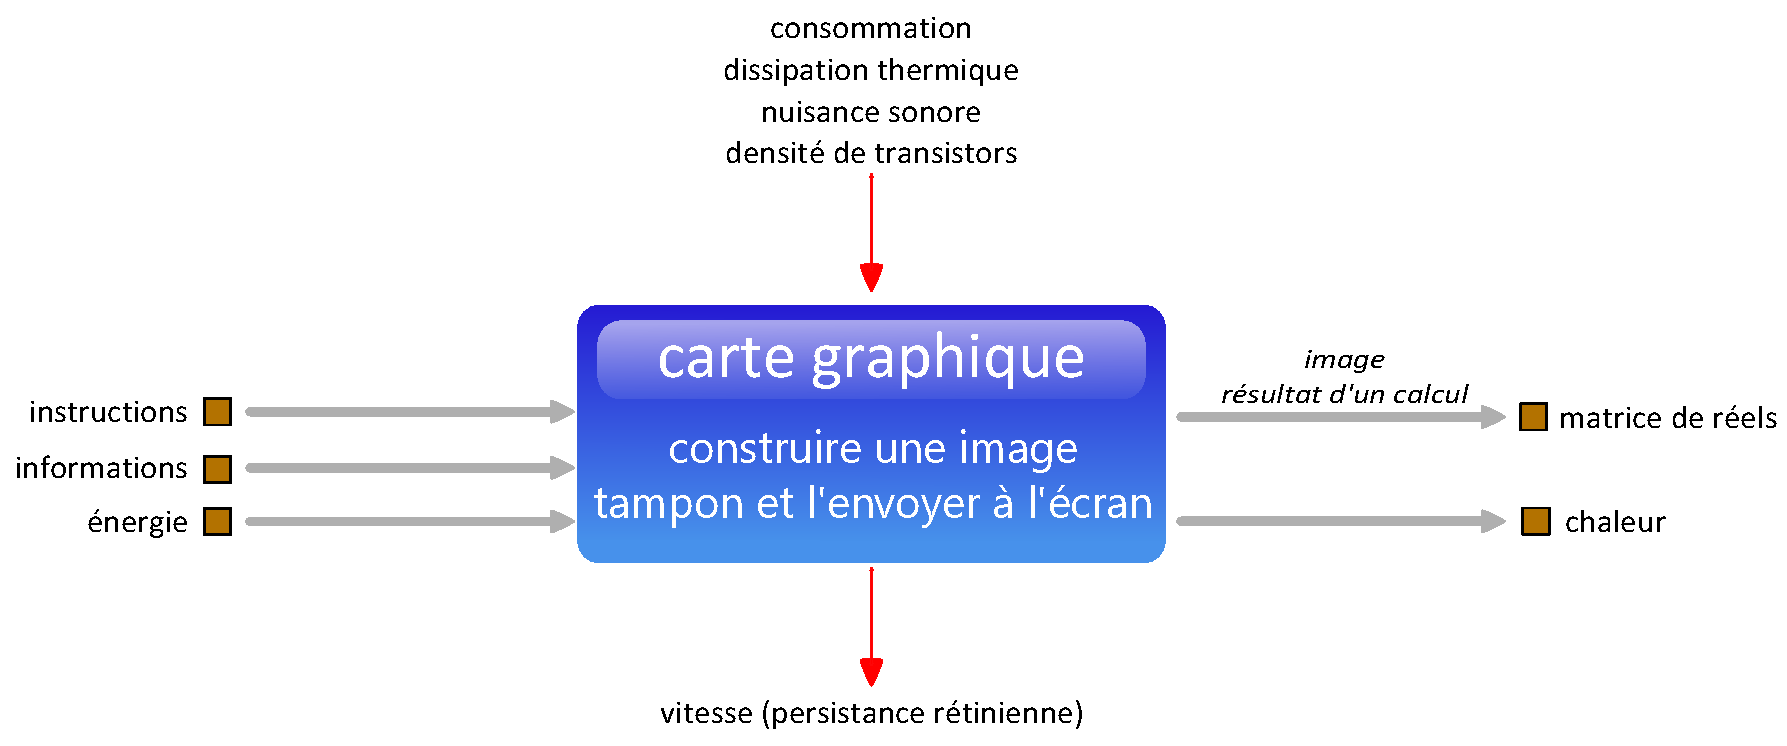
\includegraphics[width=12cm]{brique.pdf}\\
\captionof{figure}[cours]{long}
\vspace{1cm}
}
\author{AUTHORS}
\date{\today}

\hypersetup{
	pdftitle={PTITRE},
	pdfauthor={PAUTHORS},
	pdfkeywords=KEYS,
	pdflang={fr},
	pdfsubject={SUBJECT}
}

\hypersetup{
	bookmarks=true,
	unicode=true,
	pdfdisplaydoctitle=true,
	pagebackref=true
	%colorlinks=false,       % false: boxed links; true: colored links
	%linkcolor=red,          % color of internal links
	%citecolor=green,        % color of links to bibliography
	%filecolor=magenta,      % color of file links
	%urlcolor=cyan           % color of external links
}

% Divers
\parskip 10pt
\newcolumntype{M}[1]{>{\raggedright}m{#1}}
\widowpenalty=10000
\clubpenalty=10000
\renewcommand{\labelitemi}{\ding{167}}

% Tracé de courbes
\usepackage{pgfplots}
\pgfplotsset{width=\textwidth,compat=1.5}

% Glossaire
\usepackage[xindy]{glossaries}
\makeglossaries
\newacronym{deee}{DEEE}{déchet électronique et éléectrique}
\newglossaryentry{pixel} {
	name=pixel,
	description={\emph{picture element}}}



% Bibliographie
\usepackage{csquotes}
\usepackage[style=numeric,backend=biber,sortlocale=fr,date=comp,language=french,hyperref=true,useauthor=true,useeditor=false]{biblatex}
\addbibresource{rapport.bib}
%        Bibliographie d'xmemoire.cls
%% Redéfinir les mots-clefs pour la biblio, et ajouter un "art. cit."
\DefineBibliographyStrings{french}{
	opcit = \iffieldequalstr{entrytype}{article}{art\adddotspace cit\adddot}{\emph{op\adddotspace cit}\adddot},
	idem = {\emph{idem}},
	ibidem = {\emph{ibid\adddot}},
	byeditor = {\'ed\adddotspace \smartof{} },%
}
% Virgules au lieu de points dans la biblio.
\renewcommand*{\newunitpunct}{\addcomma\space}
% Tripoter le style standard pour avoir une virgule au lieu de deux points avant la date.
\renewbibmacro*{publisher+location+date}{%
\printlist{location}%
\iflistundef{publisher}
{\setunit*{\addspace}}
{\setunit*{\addcomma\space}}%
\printlist{publisher}%
\setunit*{\addcomma\space}%
\printfield{year}%
\newunit
} 
%% Il est possible de redéfinir des sections dans la biblio 
% Exemple : \defbibheading{corpus}{\subsection*{-A- Textes du corpus}}

% Pour afficher du code
\usepackage{listings}
\usepackage{textcomp}
\usepackage{setspace}
\renewcommand{\lstlistlistingname}{listings}
\renewcommand{\lstlistingname}{listing}
\definecolor{gray}{gray}{0.5}
\definecolor{green}{rgb}{0,0.5,0}
\definecolor{lblue}{rgb}{0.5,0.5,1}
\definecolor{sblue}{rgb}{0.1,0.1,0.6}
\lstnewenvironment{java}[1][]{
	\lstset{
		language=java,
		basicstyle=\ttfamily\small\setstretch{1},
		stringstyle=\color{red},
		showstringspaces=false,
		alsoletter={1234567890},
		otherkeywords={\ , \}, \{},
		numbers=left, 
		numberstyle=\tiny,
		keywordstyle=\color{sblue},
		emph={abstract,assert,boolean,break,byte,case,catch,char,class,const,continue,default,do,double,else,enum,extends,final,finally,float,for,goto,if,implements,import,instanceof,int,interface,long,native,new,package,private,protected,public,return,short,static,strictfp,super,switch,synchronized,this,throw,throws,transient,try,void,volatile,while},
		emphstyle=\color{sblue}\bfseries,
		emph={[2]true, false, null, this},
		emphstyle=[2]\color{green},
		emph={[3]import},
		emphstyle=[3]\color{blue},
		upquote=true,
		morecomment=[s]{/**}{*/},
		commentstyle=\color{green}\slshape,
		framexleftmargin=1mm, framextopmargin=1mm, frame=shadowbox, rulesepcolor=\color{lblue},#1
	}}{}


% macro pour remplacer les tabulations par un espace horizontal dans verbatim
\makeatletter
{\catcode`\^^I=\active
\gdef\verbatim{\catcode`\^^I=\active\def^^I{\hspace*{2em}}%
\@verbatim \frenchspacing\@vobeyspaces \@xverbatim}}
\makeatother
